\documentclass[draft]{agujournal2025}
\usepackage{booktabs,amsmath,amssymb,microtype,url,graphicx}
\setlength{\emergencystretch}{3em}
\newcommand{\RSeeds}{20}
\newcommand{\RRecoveryAUC}{0.87}
\newcommand{\RWithinAUC}{0.81}
\newcommand{\RRetention}{94.8}
\newcommand{\RRisk}{0.8}
\newcommand{\RGroupExcess}{14.9}
\newcommand{\RTrendGain}{69.5}
\newcommand{\REuropeStations}{16}
\newcommand{\REuropeRequested}{16}
\newcommand{\REuropeErrors}{0}
\newcommand{\REuropeCases}{4474}
\newcommand{\REuropeAirCases}{458}
\newcommand{\REuropePowerMAE}{0.846}
\newcommand{\REuropeEraMAE}{0.777}
\newcommand{\RRecordDenominator}{96}
\newcommand{\RRecordStationYears}{35}
\newcommand{\RRecordStations}{20}
\newcommand{\RRecordHalfStations}{6}
\newcommand{\RPlanTwenty}{38.9}
\newcommand{\RPlanForty}{30.6}
\newcommand{\RPlanHundred}{19.2}
\newcommand{\RPlanTwoHundred}{13.4}

\makeatletter
\def\@oddhead{\vbox to 0pt{\vss\centerline{\color{ltgray}\small working manuscript for {\it Water Resources Research}}\vskip24pt}}
\let\@evenhead\@oddhead
\makeatother
\begin{document}
\journalname{Water Resources Research}
\title{Incomplete river-temperature years: separating recovery, screening and trend inference}
\authors{[Author names]\affil{1}}
\affiliation{1}{[Affiliations]}
\authoraddr{[Corresponding author and email]}
\authorrunninghead{Ignored.}\titlerunninghead{Ignored.}
\keypoints
{Observed windows in incomplete years can contradict complete-only heat records without learned reconstruction}
{Recovery diagnostics rank danger; calibrated stochastic regression gives accuracy comparable to distribution regression}
{Group-conditional coverage and selected risk differ; independent transfer and natural-gap accuracy remain unverified}
\maketitle\par
\ifnum\RSeeds<20\noindent\textbf{Development draft: only \RSeeds{} of 20 required source analyses are currently included. Pending values and empty plots are not results.}\par\fi
\begin{abstract}
Discarding incomplete river-temperature years loses information, while daily reconstruction can distort annual heat extremes. We separate screening, estimation of the hottest 30-day mean (H30), and trend inference. Twenty repetitions redraw gaps, simulations and independent-group fitting roles in an opened archive of 581 stations and 185 groups. Comparators include overlap screening, variance-preserving and stochastic reconstruction, debiasing, distribution regression and neural imputers. Within decision-time dangerous gaps, distribution regression reduces paired mean absolute error relative to the daily plug-in by a median 21.2\%, improving in all 20 repetitions, but improves only 5.3\% over functional debiasing. Calibrated stochastic regression gives comparable point accuracy and predictive scores. Recovery diagnostics retain case-level ranking information. Observed-window lower bounds in incomplete years already exceed every complete-year H30 record at \RRecordStations{} of \RRecordDenominator{} long-record stations, directly contradicting complete-only record attribution without imputation. Retaining uncertain years improves trend precision under random missingness, while strong heat-associated missingness and non-air trend stresses expose different assumptions. Neural comparisons do not support a universal empirical sign of extreme-statistic bias. Formal conditional-conformal and semi-supervised risk-control comparisons distinguish conditional coverage, selected risk and independent-group sample requirements. Individual caps improve average-risk trade-offs but leave between-group risk; small label budgets give no useful conservative certificates. Hot-year extrapolation exposes interval miscalibration. Repetitions describe the same archive, and historical registered failures remain unchanged. Natural peak-window references and a publicly registered new-region evaluation remain unavailable. Incomplete years support question-specific inferences; single-value release needs separate validation.
\begin{plainlanguagesummary}
A gap outside a river's usual hottest period often has little effect on its annual heat statistic. A gap covering that period can remain difficult. We compared a cheap screen, classical reconstruction and learning methods, with separate rules for releasing one value and keeping uncertain years in a trend. A calibrated classical method performed about as well as the more elaborate annual model. Keeping incomplete years mainly improved trend precision. It also corrected record attribution: at some rivers, thirty consecutive reported daily values in an incomplete year were already warmer than every complete-year heat record. That conclusion requires no gap filling by this study. Low average error did not ensure safety at every river, and unusually hot years reduced interval coverage. A new regional test must be registered before its temperatures are downloaded; real outages still need suitable reference measurements.
\end{plainlanguagesummary}
\end{abstract}

\section{Introduction}
River-temperature archives support analyses of warming, heat waves and habitat suitability \cite{caissie2006,michel2020,vanhamel2024}. Annual statistics of sustained heat, including the hottest 30 consecutive days introduced as the stream thermal peak by \citeA{beaufort2022}, depend on both the observations and their missingness pattern. Completeness criteria often remove years before any annual statistic is estimated. Regression reconstruction uses more years, but an accurate daily conditional mean is not a realization of the unresolved temperature process.

The effect of regression on variability and extremes is established hydrological knowledge. \citeA{matalas1964} developed hydrological record augmentation; \citeA{hirsch1979,hirsch1982} compared regression, regression plus noise and maintenance-of-variance extension; \citeA{vogel1985} developed minimum-variance augmentation. The contribution sought here is therefore a decision-specific evaluation of annual thermal extremes, rather than discovery that deterministic regression compresses variability. Modern imputation models extend the comparison to attention-based point imputation and conditional diffusion sampling \cite{saits2023,csdi2021}.

Three distinctions determine the experimental design. Recovering one annual value differs from preserving a trend. A predictive interval differs from a point estimate. Controlling average loss in an admitted collection differs from protecting every admitted site-year. A one-feature rule based on overlap between a gap and a training-period climatological peak window is a necessary comparator, because most real calendars do not obscure that window. A learned score must show its added value among the dangerous cases that this simple rule would reject.

We ask whether recovery diagnostics add case-level information, whether annual distribution regression improves on inexpensive hydrological alternatives, and whether a change in record handling changes a scientific conclusion or mainly its precision. Previous Australian and additional USGS evaluations are opened-data development evidence after recomputation. They cannot establish independent transfer. The present revision preserves their historical registered verdicts and prepares a new public registration without requesting the proposed population's water-temperature values.

\section{Data and experimental design}
\subsection{Opened archive and observation units}
The source archive combines previously assembled European and US daily records: 581 stations, 185 connected-network groups, 27 regions and 6,170 unique complete station-years. Randomized masks produce 145,627--145,823 reconstruction cases per repetition. Daily NASA POWER air temperature supplies the common forcing \cite{nasapower2026}. Daily discharge is available at a subset of USGS stations. Analyses distinguish station identity, connected-network independence group and region. All target and donor connections represented in a held region are excluded from annual-estimator and calibration roles. A target station's other years remain available for its historical daily reconstruction, as they would in offline archive repair. This grouping controls connected-record reuse; it does not prove independent climates.

External forcing sensitivities use Daymet V4 \cite{thornton2021daymet} and ERA5-Land \cite{munoz2021era5land}, the latter served through the Open-Meteo historical API. Nearby observed-air sensitivity uses NOAA GHCN-Daily TAVG \cite{menne2012ghcn,menne2012ghcndata}. Station rosters use coordinates and record inventory without water-error screening, and raw responses and query provenance are retained. Reported air-day conventions are preserved and distinguished; POWER daily defaults to local solar time.

Forcing comparisons reuse a separate fixed set of source masks and refit the original local daily Ridge model after excluding the complete held year. Each alternative is compared on its own shared cases, while unavailable inputs remain in eligible denominators. Connected-group resampling uses 2,000 draws; it does not represent twenty mask and model repetitions.

For Northern Hemisphere stations, the analysis year is a calendar year. The established workflow uses station-specific warm seasons derived from training climatology. For the opened Southern Hemisphere comparison, translating dates by 184 days maps July--June exactly onto the following January--December, including leap years; the annual boundaries are checked explicitly. Differential split tests hold out every hot or future year from all upstream fits, including daily regressions, Air2stream calibration, air-anomaly references, climatology, residual replay and annual models. The proposed independent study also fixes July--June boundaries and daily aggregation before acquisition.

The source masking design includes 30-, 60- and 90-day gaps crossed with peak-overlap classes, and empirical incomplete calendars. Complete target-year values are used only for evaluation after masks are drawn. Decision-time features include the fraction of the climatological peak hidden, visible neighbors, known air anomalies and historical residual diagnostics. True peak overlap and true hot-year status are evaluation quantities, never admission features.

\subsection{Repeated source development and group separation}
Twenty integer seeds redraw masks, empirical-calendar choices, residual trajectories and group composition. Deterministic daily fits for a given historical training set can be shared across seeds, while all random mask and simulation streams change. Within each outer held region, remaining independent groups are randomly assigned to estimator fitting, interval calibration, failure-score learning and rule calibration. Resampling with replacement occurs within each disjoint role; a repeated copy cannot enter another role. Failure-score learning has an additional disjoint probability-calibration subset. This removes the indirect leakage that can occur when calibrating with other regions' out-of-fold predictions whose underlying models have seen the final held region.

We report the median, empirical 2.5th and 97.5th percentiles and direction counts over seeds. These empirical ranges describe algorithm and composition variation on a fixed archive, rather than confidence intervals for a new climate. Only a direction reproduced in at least 18 of 20 analyses is eligible for a quantitative abstract claim. The historical registered endpoints are listed separately in Table~\ref{tab:historical}; exploratory redesign cannot change their verdicts.

\subsection{Recovery and estimation comparators}
The recovery model approximates hidden residuals with a Gaussian autoregressive process and mixes over training-year peak positions and anomalies. Let $h_y$ and $a_y$ be the masked fraction and water-temperature anomaly of training year $y$'s peak window, $m_y=30h_y$, and $v(m,\phi)$ the variance factor for an AR(1) window mean. With residual variance $\sigma_r^2$, anomaly variance $\sigma_a^2$, and an end-contiguous hidden-window cross-covariance factor $c_y$, the window-scale approximation is
\begin{align}
\lambda_y&=\left[\frac{\sigma_r^2c_y}{\sigma_a^2v(30,\phi_a)}\right]_0^1, &
\mu_y&=h_y(\mu_r-\lambda_y a_y),\\
s_y^2&=h_y^2\max\left\{\sigma_r^2v(m_y,\phi_r)-\frac{(\sigma_r^2c_y)^2}{\sigma_a^2v(30,\phi_a)},\;0.05\sigma_r^2v(m_y,\phi_r)\right\}.
\end{align}
Here $[\cdot]_0^1$ clips to $[0,1]$ and the 5\% variance floor is explicit regularization. We equally mix component Gaussian error distributions, truncating each above $P_0-L$, where $P_0$ is plug-in H30 and $L$ the best fully observed window. Unknown target peak positions are represented by training peaks; this does not model all changes in peak selection. We call this a model because its Gaussian, stationarity and covariance approximations can fail. Its primary tests are case-level AUC and Brier skill against a leave-region lookup, within-cell AUC and diagnostic retention in the dangerous stratum. A five-degree-of-freedom Student sensitivity uses the stored nominal scale proxy; it is not a strict variance match to the truncated mixture. Cell-average explained variance does not establish unique information.

Point comparators are the priority daily plug-in, observed-day practice, a fitted lookup correction and functional debiasing. Classical comparisons include annual and warm-season MOVE.1 daily completion and annual H30 augmentation. MOVE.1 preserves training mean and variance for the fitted proxy; it does not reproduce unresolved temporal dependence. Stochastic regression adds twenty conditional AR(1) residual bridges, conditioned on available gap endpoints. Its annual target is calculated separately for every draw.

Distribution regression learns quantiles of the plug-in's annual error and calibrates them by decision-time difficulty on independent groups. The stochastic-regression and state-simulation distributions receive the same calibration groups, bootstrap multiplicities and difficulty offsets, so calibration access cannot explain an apparent advantage. Point estimates use medians. No interval is invented for a deterministic method. For sampled paths, H30 is calculated before summarizing their distribution. The fixed-architecture CPU comparisons use MSE boosting, a cross-station MSE LSTM, SAITS and CSDI, sharing three group splits and identical test masks within each split. Additional boosting arms use the ridge model's air lags and available discharge. Neural inputs omit neighbor series, so comparisons of algorithm performance emphasize the air-ridge tier. Missing flow means unavailable prediction. These are specified comparator budgets, not exhaustive searches or best available neural performance.

The globally fitted neural comparators use local other-year history for climatology, while classical daily models also refit a local water--air relation. Their accuracy differences therefore include adaptation strategy. For the Jensen mechanism we additionally report the mean of the sampled H30 values: its target differs from the median used for MAE, and from H30 of the mean daily path.

A separate locally fitted nonlinear MSE control uses exactly the ridge air lags and annual harmonics, with all held-year water values excluded from training. Its flow arm adds available log-discharge lags. This matches the local fitting scope rather than attributing all global-versus-local differences to model architecture; a held-year perturbation test verifies the exclusion.

The conditional-mean mechanism has a precise theoretical form. For window means $w_j^\top Y$ and observed information $X$, convexity gives
\begin{equation}
\max_j w_j^\top E(Y\mid X)\;\leq\;E\{\max_j w_j^\top Y\mid X\}.
\end{equation}
This statement concerns the true conditional mean and conditional expected H30. Approximate regressions can have additional positive or negative errors; it does not predict the sign of every observed case, nor guarantee that a finite diffusion model has calibrated tails.

\subsection{Scoring and decision rules}
Scores are reported for all cases and by decision-time overlap bin, information tier and air-indicated hot condition. Point metrics are MAE and failure probability beyond 0.5$^{\circ}$C. Distribution metrics are CRPS, 90\% interval score, coverage and width \cite{gneiting2007,romano2019}. Upper-tail CRPS uses the training-period H30 90th percentile as a threshold, with the transformation $v(x)=\max(x,u)$ applied to forecasts and outcomes. Every case remains in this proper-score calculation \cite{gneiting2011weighted,lerch2017}. The stored quantiles are integrated through 128 midpoint samples of a piecewise-linear quantile function with constant outer tails. This is a documented approximation to the fitted full distribution, applied equally across quantile-based arms; the residual bridge has an exact empirical-ensemble CRPS.

Individual release uses $p_i\leq c$, with prespecified sensitivity caps. For false admission cost $L_b$ and false rejection cost $L_g$, the score-based Bayes decision is $p_i\leq L_g/(L_b+L_g)$ when probabilities are calibrated. Relative economic value compares each decision with the better of retaining or rejecting every case \cite{richardson2000}. Batch-average admission is evaluated both alone and with a maximum individual probability. We also compare application within independent groups, empirical overlapping-group post-calibration and a random-effects log observed/expected ratio with a new-region prediction interval \cite{riley2016}. Empirical group adjustments do not implement or inherit the guarantees of a formal conditional-calibration method.

An independent-group bounded-loss certificate provides a distinct, conservative comparator. Its threshold family and score are fixed before calibration. The target is selected risk under uniform sampling of a new group and a stated within-group sampling scheme, not every group's conditional risk. Unsupported nonempty admission is reported as insufficient evidence. Local-label curves report certificate status, realized risk and retention separately. Prior EM, importance weighting, average confidence, ATC and prediction-powered residual corrections are assumption-dependent diagnostic comparisons; none automatically certifies transfer under arbitrary conditional shift.

We additionally implement the finite-basis conditional conformal method of \citeA{gibbs2025conditional}, including conservative and casewise independently randomized prediction sets for the binary failure label. The binary LAC score is $|Y-p(X)|$, where $p$ is the frozen failure score. Calibration uses one uniformly chosen case per independent group; repeated masks do not inflate its sample size. Overlapping indicators represent macro-region, tier, peak overlap, historical heat and available river proxies. A full held-region indicator has no source support. Release occurs only for the singleton set containing ``no failure.'' Conditional prediction-set coverage bounds false-admission frequency, so
\[
 P(F\cap A\mid G)\leq\alpha
 \quad\Longrightarrow\quad
 P(F\mid A,G)\leq\alpha/P(A\mid G),
\]
when admission has positive probability. It does not bound selected risk by $\alpha$. We also evaluate general-loss semi-supervised RCPS with finite-sample WSR bounds \cite{einbinder2025semi}, using distinct labeled, unlabeled-calibration and test groups. The group loss $B_g+r(1-A_g)$ targets $E(B_g)/E(A_g)\leq r$; its validity requires same-population independent groups and a fixed predictor. Held-region shift need not satisfy the conditional-conformal exchangeability assumption.

\subsection{Scientific-use tests}
Trend experiments compare discarding incomplete years, a 90\% warm-season criterion, retaining plug-in values, multiple imputation and a lower-bound likelihood. A fully observed 30-day window gives a lower bound $L$ for H30, so its likelihood contribution is a survival probability $P(H30\geq L)$. This is right censoring of the response. It is a Gaussian working likelihood inspired by interval-data reasoning, not Bulletin 17C's expected moments algorithm \cite{england2019}. Window bounds can be informative, so consistency is not assumed.

The heat-associated stress assigns missing-year probabilities 0.90 and 0.18 to the hottest air-indicated tenth and other years. Random missingness matches its station-specific marginal probability. An annual-target sensitivity adds 0.2$^{\circ}$C per decade without adapting previously fitted imputations, deliberately testing incompatibility. A distinct three-seed daily experiment adds this component to all complete daily target and donor water records, keeps air unchanged, and refits every upstream stage. This tests whether a smooth non-air trend can be learned from history; it is not an abrupt unseen regime shift. We report bias-squared and variance contributions, station RMSE ratios and exact deletion counts. Multiple imputations sample independently across years and use Rubin combining rules with a finite-degrees-of-freedom adjustment; missing-component and total trend intervals are distinguished.

A separate unflagged-exposure stress replaces seven consecutive visible warm-day readings with concurrent air temperature. The window is drawn from the hottest tenth of eligible air windows, without hidden water values. Three mask and trajectory seeds retain clean source-fit seed zero, its failure classifier and interval calibration. The target remains a defined water temperature; no physical water temperature is assigned to a genuinely dry bed. The fixed-severity scenario does not estimate the archive prevalence of exposure.

The actual archive comparison reports station eligibility under completeness criteria and retention with estimation. It includes same-station contrasts to distinguish roster changes from changes in annual support. Regional medians use independent-group resampling. Station-level trend tests are accompanied by false-discovery adjustment and synchronized temporal-null resampling. Hot-year comparisons report hits, false alarms and SEDI. The analyzed panel is an assembled archive; it is not a census of all USGS water-temperature sites.

For record attribution we use an observation-only check. Among stations with at least fifteen complete observed years in 1981--2025, let $M_s$ be the maximum complete-year H30. Every complete thirty-day window in an incomplete year gives $H30_{sy}\geq L_{sy}$. If $L_{sy}>M_s$, the complete-only record cannot be the full-record maximum. We recompute all complete-year references and every window witness from original input daily values. This deterministic statement concerns reported series, without imputation or random seeds; it does not identify the unique warmest incomplete year or remove measurement error. Additional same-roster regional comparisons use identical first-to-last-complete-year spans, report common versus expanded year sets, and require 80\% fixed-roster support for annual regional means.

\section{Results}
\subsection{Triage and the information in recovery diagnostics}
Figures~\ref{fig:triage} and \ref{fig:recovery} separate risk concentration from case discrimination. The median recovery-model AUC under controlled gaps is \RRecoveryAUC{}, compared with 0.785 for the lookup, with within-cell AUC \RWithinAUC{}. Dangerous-stratum AUC remains 0.784. Ranking at a diagnostic 5\% realized risk retains approximately 24\% of dangerous controlled cases using the recovery model and 36\% using the distribution-regression failure score. These evaluation-label-based frontiers are not deployable thresholds or calibrated tail probabilities. The one-feature screen retains approximately 92\% of empirical-calendar cases, establishing a strong inexpensive benchmark before learning is considered.

\subsection{Point estimates and distributions}
Figure~\ref{fig:estimators} compares common dangerous cases. Distribution regression improves paired MAE over the plug-in by a median 21.2\% (empirical repetition range 20.6--22.4\%), with improvement in 20/20 repetitions. Improvement over functional debiasing is only 5.3\% (3.9--6.6\%); none reaches the specified 10\% material-improvement threshold. It beats raw stochastic regression in only 6/20 repetitions. Median single-arm dangerous-stratum MAEs are 0.428, 0.355, 0.337 and 0.336$^{\circ}$C for plug-in, functional debiasing, distribution regression and calibrated stochastic regression, respectively; paired effects retain common-case availability.

Raw stochastic-regression interval coverage is 75.3\%, increasing to 89.2\% after disjoint-group calibration; distribution-regression coverage is 88.8\%. Calibrated stochastic regression has median CRPS 0.247 and interval score 2.105$^{\circ}$C, compared with 0.248 and 2.123 for distribution regression. On common cases, distribution regression improves CRPS in only 7/20 repetitions and improves upper-tail CRPS in none. Thus neither unique point nor unique distributional value is established. The redesigned raw P1 analogue passes in 0/20 repetitions, whereas its calibrated analogue passes in 20/20; neither changes historical P1's failure.

Among matched dangerous air-ridge cases in three group splits, median H30 MAE is approximately 0.460$^{\circ}$C for SAITS, 0.531 for CSDI, 0.479 for LSTM and 0.490 for lagged-air boosting. Their signed biases vary in direction; neither universal cold bias of point models nor its universal removal by sampling is supported. These small fixed-budget comparisons constrain the mechanism claim without ranking optimally trained model families.

Using the sampled functional mean for CSDI, signed biases in the three air-ridge splits are approximately $-0.093$, $-0.003$ and $+0.430^{\circ}$C. Changing the point summary does not give a universal empirical sign. Jensen's inequality describes the exact conditional mean under a specified distribution; approximate global imputation, local adaptation and distributional calibration remain separate empirical questions.

\subsection{Admission and scientific use}
The source-fixed individual cap of 0.10 retains a median \RRetention\% of real-calendar cases at \RRisk\% realized failure. Poststratification to historically supported incomplete station-years gives approximately 943 retained and 5.8 failures per 1,000; a 50\% overlap screen using the same delivered estimator gives 925 retained and 4.7 failures. Unsupported strata remain in the denominator. These opened-source estimates describe a trade-off, not a universal preference. Figure~\ref{fig:decisions} shows cost dependence. Under controlled gaps, the individual cap retains 76.8\% at 5.21\% risk, but \RGroupExcess\% of evaluable groups exceed 10\% risk (Figure~\ref{fig:group}). Empirical group adjustment reduces this excess fraction to 2.7\% while losing 15 percentage points of retention, exceeding the planned five-point allowance.

This adjustment combines a global probability map and empirical group factors. With the same cap and predictions, Platt calibration alone retains 63.8\% of controlled-gap cases, with 3.2\% of evaluable groups above 10\% risk; adding group factors retains 61.8\%, with 2.7\% above the limit. The entire change from raw scores cannot be attributed to overlapping-group adjustment.

The conservative group certificate remains empty under source calibration and every evaluated 2--16-group local-label budget. This is insufficient independent-group evidence, rather than successful risk control. Joint E1/E2 planning uses all twenty source repetitions and 40,000 empirical group simulations per budget. The equal-seed mixture passes with probability \RPlanTwenty\% at twenty groups, \RPlanForty\% at forty and \RPlanTwoHundred\% at two hundred. Seed-to-seed variation is substantial. No tested budget reaches the 80\% planning criterion; these simulations do not establish new-climate power. The candidate supports a failure-detection study rather than a promise that sample size alone will certify transfer.

The formal semi-supervised RCPS comparison also gives no nonempty certificate at these label budgets. At eight or more labeled groups, the evaluated regional pools additionally lack enough distinct unlabeled calibration groups while retaining an untouched test pool. Conservative conditional conformal sets are uninformative at the chosen overlapping-group resolution. Randomized versions are evaluated separately: their set coverage and false-admission frequency must be assessed alongside selected risk, rather than relabeled as safe single-value release. Requiring a previously unseen regional group yields no singleton release. Supplementary tables report calibration support, numerical fallbacks and the two risks separately.

Figure~\ref{fig:downstream} separates trend error from hot-event classification. The median random-missingness trend RMSE reduction relative to the warm-season rule is \RTrendGain\%, with improvement in 20/20 repetitions; the strong-heat stress gives 69.6\%. Approximately 95\% of the warm-season rule's random-missingness mean squared error is variance. The result primarily supports precision and information retention. A median 31 station deletions is required to reverse the random-missingness comparison. The incompatible annual non-air sensitivity reverses the advantage in all 20 repetitions, with median RMSE 60\% greater than the warm-season rule. In the separate daily-process refit, three-seed pooled RMSE is approximately 0.012 versus 0.039$^{\circ}$C per decade. History can accommodate this smooth added trend, but obsolete annual imputations cannot.

The missingness-component uncertainty remains inadequate. Its nominal 95\% coverage has a median 79.2\% under matched random missingness and 79.6\% under strong heat-associated missingness, despite total trend intervals covering almost 100\%. Calibrated stochastic imputation gives approximately 72.5\% and 72.7\% missing-component coverage. Applying the original numerical P4 gates to the redesigned stress analogues yields 0/20 joint passes. This does not change historical P4's verdict. Annual marginal calibration and reduced trend RMSE have not established calibrated joint trend-error uncertainty.

Within the assembled archive, station eligibility increases from 98 under complete-year selection to 255 under retention with estimation. In the USGS panel the counts are 36 and 163, and regional median slopes are 0.246 and 0.138$^{\circ}$C per decade. Among the 36 common stations, the median slope contrast is only $-0.0026$; the roster and annual support therefore require separate interpretation. A synchronized circular-shift field-test sensitivity changes from $p=0.057$ to $p=0.0005$ in this panel. Most European regional warming conclusions persist. More significant station tests and changed rosters do not establish a universal reversal of a regional scientific conclusion; incomplete-year outcomes remain unknown.

There is nevertheless a directly observed change in record attribution. At \RRecordStations{} of \RRecordDenominator{} eligible long-record stations, \RRecordStationYears{} incomplete years contain fully observed thirty-day windows exceeding every complete-year H30; \RRecordHalfStations{} stations exceed the complete-year record by more than 0.5$^{\circ}$C (Table~\ref{tab:observed-record-main}). For example, an observed 2010 window at USGS 02458450 exceeds its maximum complete-year H30 by 1.20$^{\circ}$C, and a 2018 window at Bavarian station 11401009 exceeds it by 1.15$^{\circ}$C. Every witness is verified against the original daily input. These observations invalidate the complete-only record attribution; another incomplete year could still be warmer. Learned annual reconstruction is unnecessary for this one-sided scientific conclusion.

With the same station rosters and time spans, the point-ranked hottest regional year changes from 2022 to 2018 in Bavaria, 2011 to 2010 in the HUC03 panel, and 2020 to 2012 in HUC04. The original top year persists in all three when restricted to common supported years. The change chiefly reflects newly included years. Group-bootstrap and imputation sensitivities are descriptive; HUC04 has only two independent groups, and estimated incomplete outcomes do not verify a new physical regional record.

Frozen-admission deletion audits complement the trend check. For empirical calendars, removing a median 150.5 of 185 groups is necessary to erase the individual-cap rule's retention advantage over the best qualifying published rule. Controlled-gap batch-average rules already exceed the 5\% risk criterion. The historical opened USGS N1 risk crosses its original 7\% boundary after ten of forty groups are removed from either frozen admission set, but reapplying the batch rule at those witnesses remains below the boundary. This is not an exact robustness result for rerunning the entire decision pipeline, and historical N1 retains its original verdict.

The metadata-fixed national USGS extension attempts all 1,273 candidates within a 4,285-site catalog. The retrieved annual panel contains 933 sites, with eligibility unresolved for 340 candidates. At least fifteen statistic years are available at 100 sites under complete-year selection and 521 under retention with estimation. Occupied one-degree station cells increase from 49 to 207. Network median slopes are 0.245 and 0.218 degrees C per decade; the same-roster/span median contrast is 0.0026. Both rules retain field-significant network warming in the synchronized sensitivities. Observed thirty-day windows exceed the complete-year record at 43 sites in 70 incomplete station-years. These network descriptions retain unknown-eligibility bounds; they neither represent all US rivers nor validate natural-gap imputation accuracy. Supplementary files report spatial coverage, hot-year frequency, same-roster contrasts and field significance.


% ZERO_FLOW_MISSINGNESS_BOUNDARY
The historical missingness sample includes 21 USGS sites with recorded approved zero flow. Their temperature--incompleteness odds ratio is 1.21, with a group-bootstrap interval of 0.88--1.56. This imprecise proxy analysis permits stronger associations and does not classify intermittent rivers; archive-average associations cannot establish dry-bed sensor validity.

\subsection{Driver, metric and transfer boundaries}
The forcing sensitivity covers all 319 benchmarkable USGS source sites. Original source panels, forcing and daily-model code reproduce all 67,316 POWER control cases exactly. Among 9,271 paired dangerous air-ridge cases, Daymet changes MAE from 0.661 to 0.682$^{\circ}$C. Adding discharge changes MAE from 0.708 to 0.623 in a separate 7,048-case comparison; 71\% of paired sites improve or tie. Each input has its own common-case reference. Daymet uses the midpoint of daily minimum and maximum air temperature, so product and aggregation change together; unavailable dates and calendar lags remain explicit. Nearby observed-air matching finds metadata-eligible TAVG stations within 25 km for 147 sites. Among 3,010 paired dangerous air-ridge cases at 112 sites, MAE changes only from 0.678 to 0.671$^{\circ}$C; about 51\% of paired sites improve. These observations are neither perfectly co-located nor uniformly clock-matched, and source S TAVG represents UTC-ending days. A European ERA5-Land sensitivity obtains \REuropeStations{} of \REuropeRequested{} prespecified stations. Its \REuropeCases{} paired cases include \REuropeAirCases{} dangerous air-ridge cases, with MAE changing from \REuropePowerMAE{} to \REuropeEraMAE{}$^{\circ}$C. These results do not establish universal forcing superiority. Approved daily maximum water temperature supplies 5,913 cases at 34 sites for a distinct 7DADM sensitivity, without regulatory certification.

A separate native H7 analysis repeats generation and annual/risk calibration over twenty seeds and 540 outer-region fits. H7 is the annual maximum of seven-day means of daily mean water temperature, distinct from 7DADM. In matched controlled dangerous cases, distribution regression reduces MAE by a median 2.9\% relative to calibrated stochastic regression; CRPS and upper-tail CRPS improve in all twenty repetitions. The relative advantage therefore depends on the target statistic. H7 trend missing-component coverage remains about 81\%, so this small annual-score gain does not repair trend uncertainty or change the historical H30 verdicts.

Cold-to-hot evaluation holds out the hottest 20\% of years before all upstream fitting. Distribution-regression dangerous-stratum coverage falls to 73.8\%, versus 80.4\% for calibrated stochastic regression. Training before 2010 gives approximately 84.3\% coverage for distribution regression. Source-domain interval calibration therefore does not protect hot-year or temporal extrapolation.

With clean outer-region fits from source repetition zero and three mask and trajectory seeds, unflagged air exposure raises calendar-case selected failure from a median 0.7\% to 36.9\%, while retention remains 95.0\%. Controlled-case selected failure rises from 4.9\% to 37.9\%. Under strongly heat-associated missingness, distribution-regression MI missing-component coverage falls to 16.1\%, and its RMSE reduction relative to the warm-season rule falls to about 8\%. These are synthetic measurement-contamination results, not three model fits or a twenty-repetition stability claim. Quality checks on visible observations must precede release and trend inference.

Previous Australian and new-USGS results remain supplementary opened-data checks. Metadata-only screening excludes the current Horizons public archive for insufficient calendar support and fixes nine prospective Greater Wellington sites in three conservatively merged management zones. Native clock, strict quality rules, source weights and analysis code are prepared for a small failure-detection study; complete-reference eligibility remains unverified. There is no publicly accepted OSF registration or new river-temperature outcome evaluation. Three zones cannot support the ten-labeled-group endpoint or establish general transfer. Natural reference searches produce no case satisfying both historical support and reference-quality requirements for a difficult peak-window outage. Their exclusion reasons and minimum independent-gap sample calculation are reported as a qualification result, not as verified recovery accuracy.

\section{Discussion}
The operationally useful object is a triage system with different actions for annual-value release and statistical inference. A cheap geometric screen establishes a strong lower benchmark. Learned scores can be justified by what they recover within its rejected stratum, or by a better cost-sensitive trade-off, rather than by an average dominated by easy cases. A good distribution need not be the best point prediction, and retaining uncertain years can improve trends even when some single values should be withheld.

Variance-preserving record augmentation is essential context for this argument \cite{hirsch1982,vogel1985}. The nonlinear maximum of a conditionally averaged series provides a clear mechanism, but it does not identify all model error in a specific river. Residual distributions can miss local thermal anomalies; groundwater, regulation, lake outlets and intermittent flow cannot be inferred from the sign of a regression residual alone. Improved discharge or meteorological input can therefore matter more than a more elaborate annual estimator at a particular site.

Group risk prevents a misleading interpretation of a successful archive-average rule. An average-risk prefix can admit a high-probability case because many easy cases subsidize it. An individual cap removes that decision feature while leaving calibration uncertainty intact. A random-effects prediction interval makes heterogeneity visible; a very wide interval is a reason to withhold a transfer claim. Small local label budgets must be evaluated at the independent-group level, where conservative certification may remain unavailable.

The strongest limits are empirical. Masked complete years may not represent actual sensor failure. Suitable natural peak-window references were not found among 180 candidate pair-years. Nearby NOAA observations add a meteorological comparison, but not a perfect riverbank-air or timing oracle; unavailable cases remain explicit. European high-resolution forcing evidence remains a partial sample. The failure map uses 581 station coordinates and historical GAGES-II dam metadata; zero-flow days are a proxy and lake-outlet classification has only one explicit agency designation. The source-distance screen does not flag Big Sandy Creek. Current-vintage data do not constitute an archived real-time field trial. The daily non-air refit tests a smooth historical component, not an unseen regime shift. A separate national USGS source intake now combines numeric acquisition and availability, while retaining its earlier dates-only audit. The retrieved-panel analysis retains unresolved eligibility bounds and is not new independent validation. Provisional observations remain distinct from absent data. Archive selection remains a panel analysis, and repeated use remains exploratory.

\section{Conclusions}
Archive analysis should separate recovering a value, releasing it and answering a scientific question. Retaining incomplete years improves precision and can overturn complete-only record attribution using observed windows alone. Cheap overlap rules, classical variance-preserving completion and lower-bound methods are necessary comparators. Proper scores, independent-group sample accounting and the distinction between conditional coverage and selected risk constrain stronger claims about distribution regression and transfer. Public registration before new water-temperature value access, followed by both overall and group-risk endpoints, remains necessary to close independent transfer.

\section*{Open Research}
The producing scripts, configuration, case-level scorecard, role assignments and repetition summaries are preserved in the accompanying repository. The frozen source-only candidate and code-and-protocol archive are registration materials, explicitly unregistered until publicly accepted with matching attachments. Author, affiliation, funding and permanent deposit fields are reserved for the authors to complete. No journal submission has been made.

\begin{table}[p]
\caption{Historical registered verdicts. The redesign cannot revise them.}
\label{tab:historical}
\centering\small
\resizebox{\textwidth}{!}{%
\begin{tabular}{ll}
\toprule
endpoint & verdict \\
\midrule
P1 & not met \\
P2 & not met \\
P3 & not met \\
P4 & met historically \\
N1--N3 & met after recomputation \\
\bottomrule
\end{tabular}
}
\end{table}
\begin{table}[p]
\caption{Exploratory direction stability; positive differences favor distribution regression. MAE and trend entries are fractional reductions; CRPS entries are score differences in degrees C. These are repeated analyses of the same archive.}
\label{tab:stability0}
\centering\small
\resizebox{\textwidth}{!}{%
\begin{tabular}{lllll}
\toprule
metric & comparison & positive & repeats & median \\
\midrule
MAE reduction & Daily plug-in & 20 & 20 & 0.212 \\
MAE reduction & Functional debiasing & 20 & 20 & 0.053 \\
MAE reduction & Lookup debiasing & 20 & 20 & 0.202 \\
MAE reduction & Annual MOVE.1 & 20 & 20 & 0.263 \\
MAE reduction & Warm-season MOVE.1 & 20 & 20 & 0.243 \\
MAE reduction & Stochastic regression & 6 & 20 & -0.003 \\
MAE reduction & Calibrated stochastic & 11 & 20 & 0.002 \\
MAE reduction & Calibrated state & 20 & 20 & 0.072 \\
CRPS improvement & Calibrated state & 20 & 20 & 0.017 \\
Tail CRPS improvement & Calibrated state & 20 & 20 & 0.004 \\
CRPS improvement & State simulation & 20 & 20 & 0.018 \\
Tail CRPS improvement & State simulation & 20 & 20 & 0.004 \\
\bottomrule
\end{tabular}
}
\end{table}
\begin{table}[p]
\caption{Exploratory direction stability; positive differences favor distribution regression. MAE and trend entries are fractional reductions; CRPS entries are score differences in degrees C. These are repeated analyses of the same archive.}
\label{tab:stability12}
\centering\small
\resizebox{\textwidth}{!}{%
\begin{tabular}{lllll}
\toprule
metric & comparison & positive & repeats & median \\
\midrule
CRPS improvement & Stochastic regression & 12 & 20 & 0.001 \\
Tail CRPS improvement & Stochastic regression & 0 & 20 & -0.001 \\
CRPS improvement & Calibrated stochastic & 7 & 20 & -0.001 \\
Tail CRPS improvement & Calibrated stochastic & 0 & 20 & -0.001 \\
Trend RMSE reduction & mcar & 20 & 20 & 0.695 \\
Trend RMSE reduction & non air trend & 0 & 20 & -0.602 \\
Trend RMSE reduction & strong heat & 20 & 20 & 0.696 \\
\bottomrule
\end{tabular}
}
\end{table}
\begin{table}[p]
\caption{Observed-window record attribution on reported daily series, with no imputation. The eligible population contains 96 stations and at least fifteen complete observed years per station in 1981--2025. Positive excess means the complete-only record cannot be the full-record maximum.}
\label{tab:observed-record-main}
\centering\small
\resizebox{\textwidth}{!}{%
\begin{tabular}{llll}
\toprule
margin c & n station years & n stations & n groups \\
\midrule
0.000 & 35 & 20 & 15 \\
0.500 & 12 & 6 & 6 \\
1.000 & 3 & 2 & 2 \\
\bottomrule
\end{tabular}
}
\end{table}

\begin{figure}[p]\centering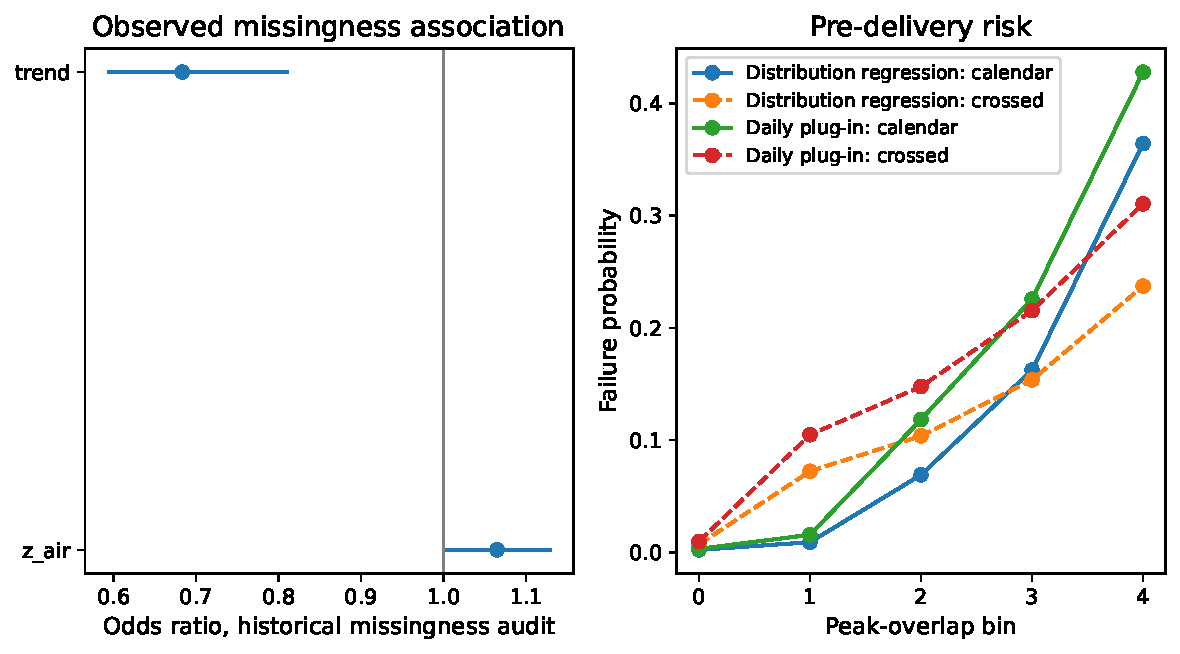
\includegraphics[width=.85\textwidth]{figures/review_completion/r4_1_missingness_triage.pdf}\caption{Decision-time risk concentration across peak-overlap bins. Source tables preserve populations, layers and repetition variability.}\label{fig:triage}\end{figure}
\begin{figure}[p]\centering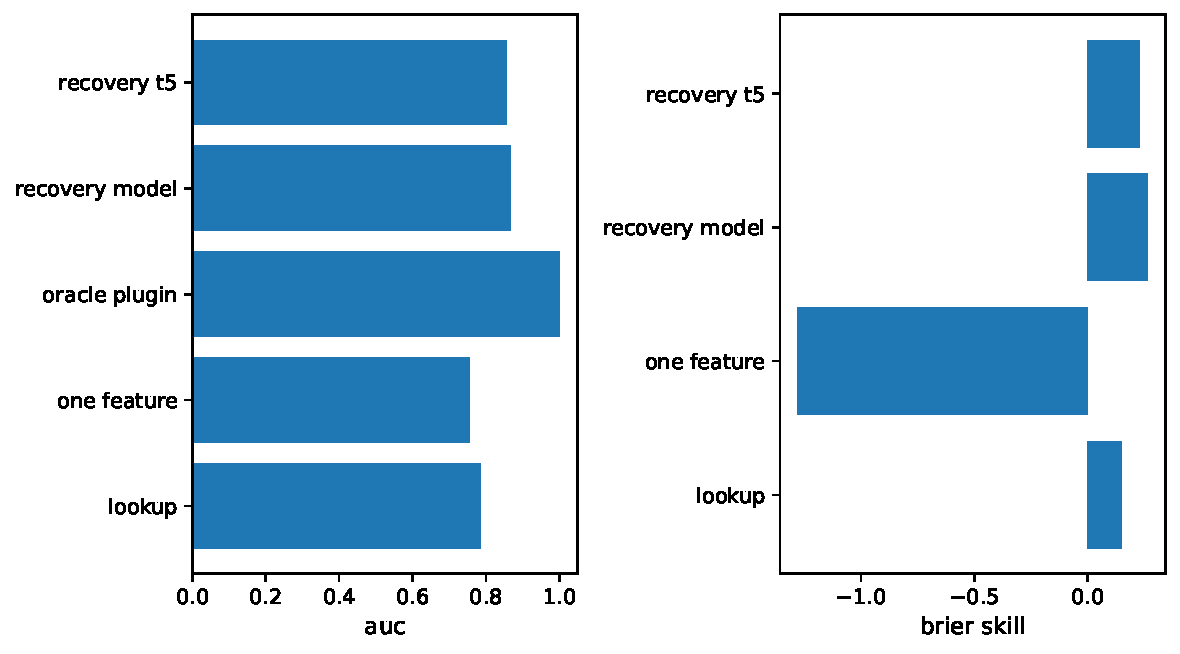
\includegraphics[width=\textwidth]{figures/review_completion/r4_2_recovery.pdf}\caption{Recovery-model discrimination and Brier skill against simple scores. Ranking does not imply calibration.}\label{fig:recovery}\end{figure}
\begin{figure}[p]\centering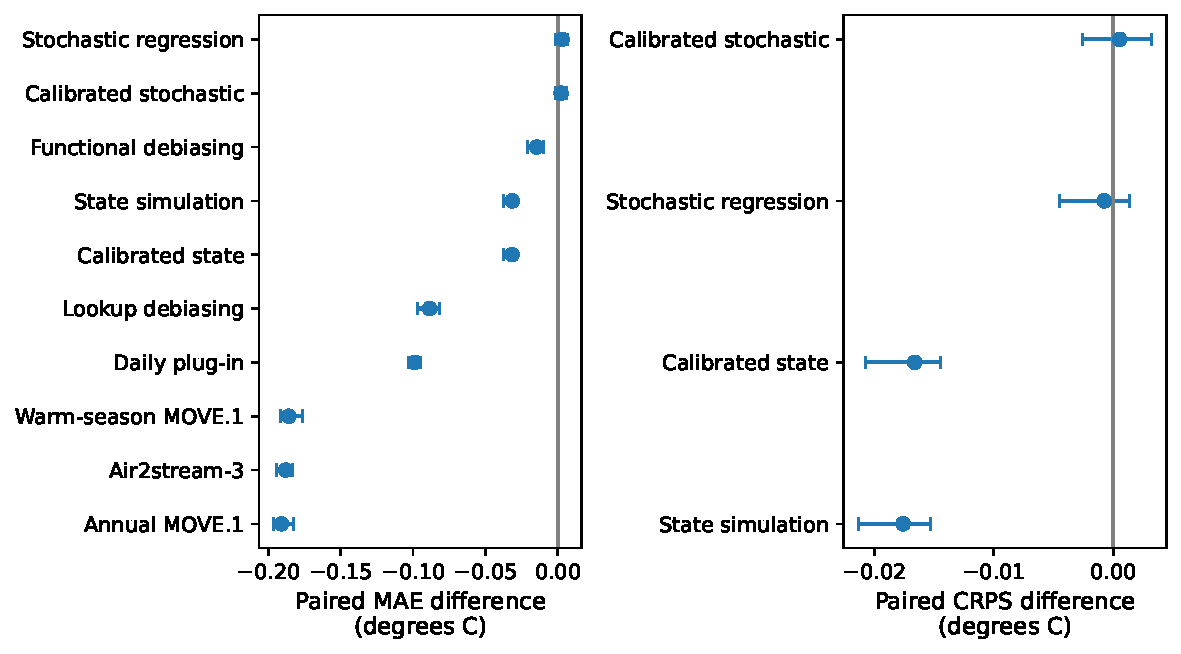
\includegraphics[width=\textwidth]{figures/review_completion/r4_3_estimators.pdf}\caption{Dangerous-case paired point and distribution scores. Negative differences favor distribution regression. Points are repetition medians; bars are empirical 2.5th--97.5th percentiles over the same opened archive, not population confidence intervals. Deterministic methods have no invented distributions.}\label{fig:estimators}\end{figure}
\begin{figure}[p]\centering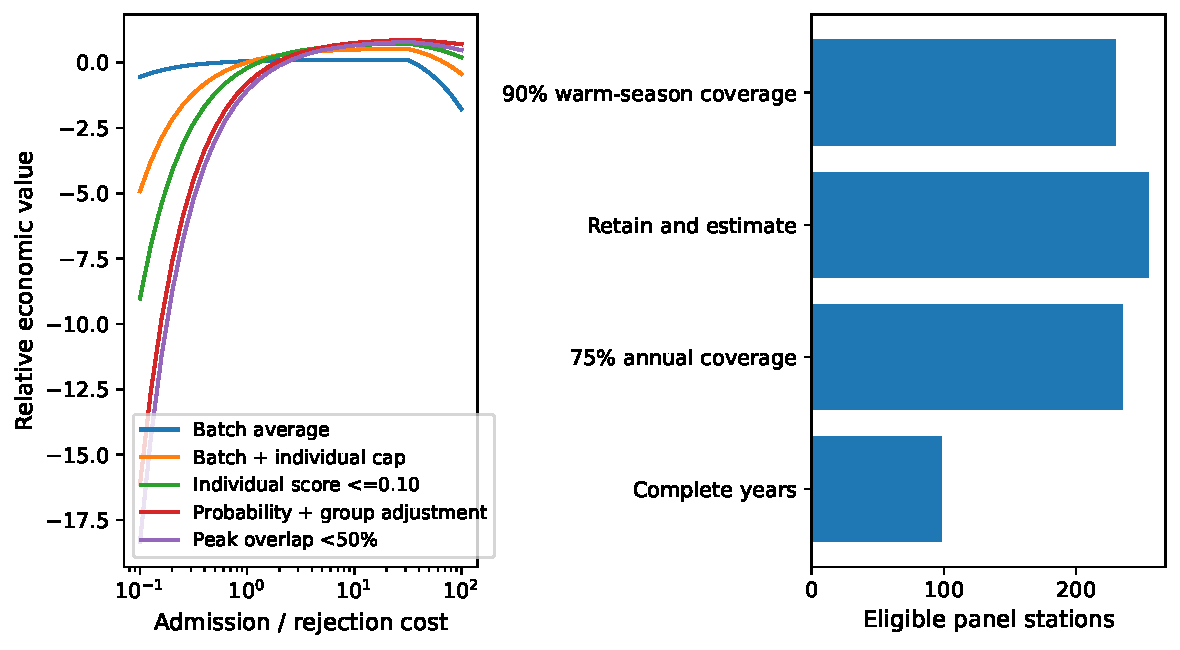
\includegraphics[width=\textwidth]{figures/review_completion/r4_4_decisions_selection.pdf}\caption{Decision cost sensitivity and station eligibility in the assembled archive.}\label{fig:decisions}\end{figure}
\begin{figure}[p]\centering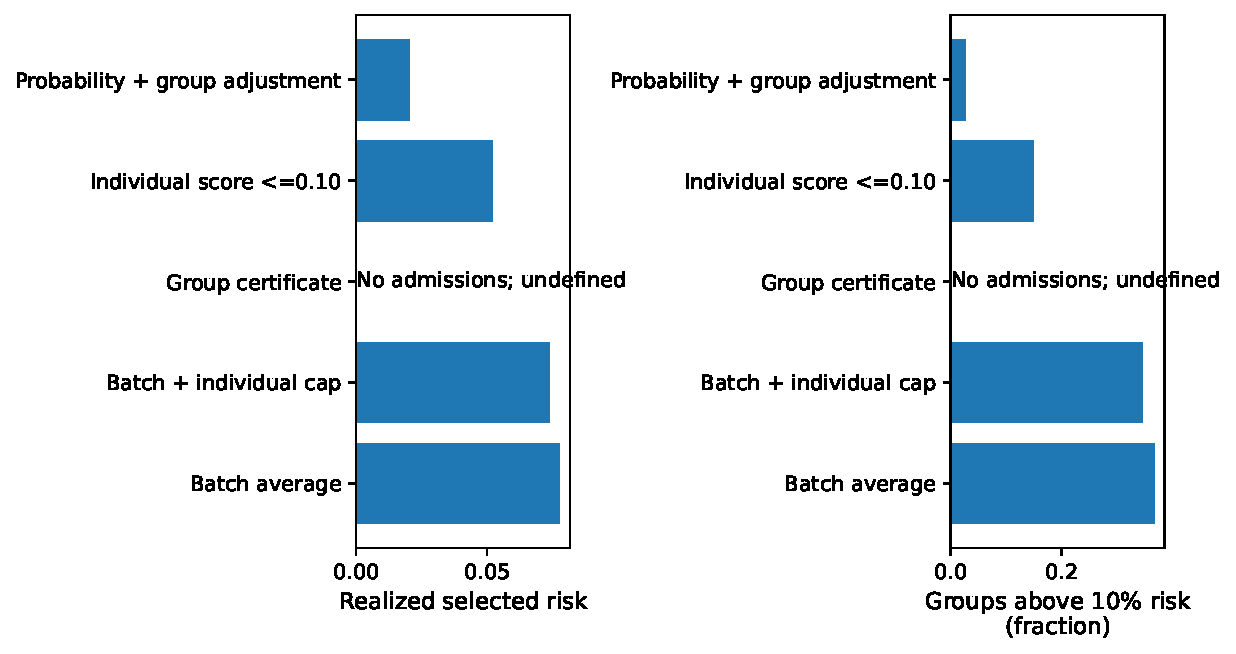
\includegraphics[width=\textwidth]{figures/review_completion/r4_5_group_risk.pdf}\caption{Average risk and the fraction of evaluable groups with risk above 10\%, reported separately.}\label{fig:group}\end{figure}
\begin{figure}[p]\centering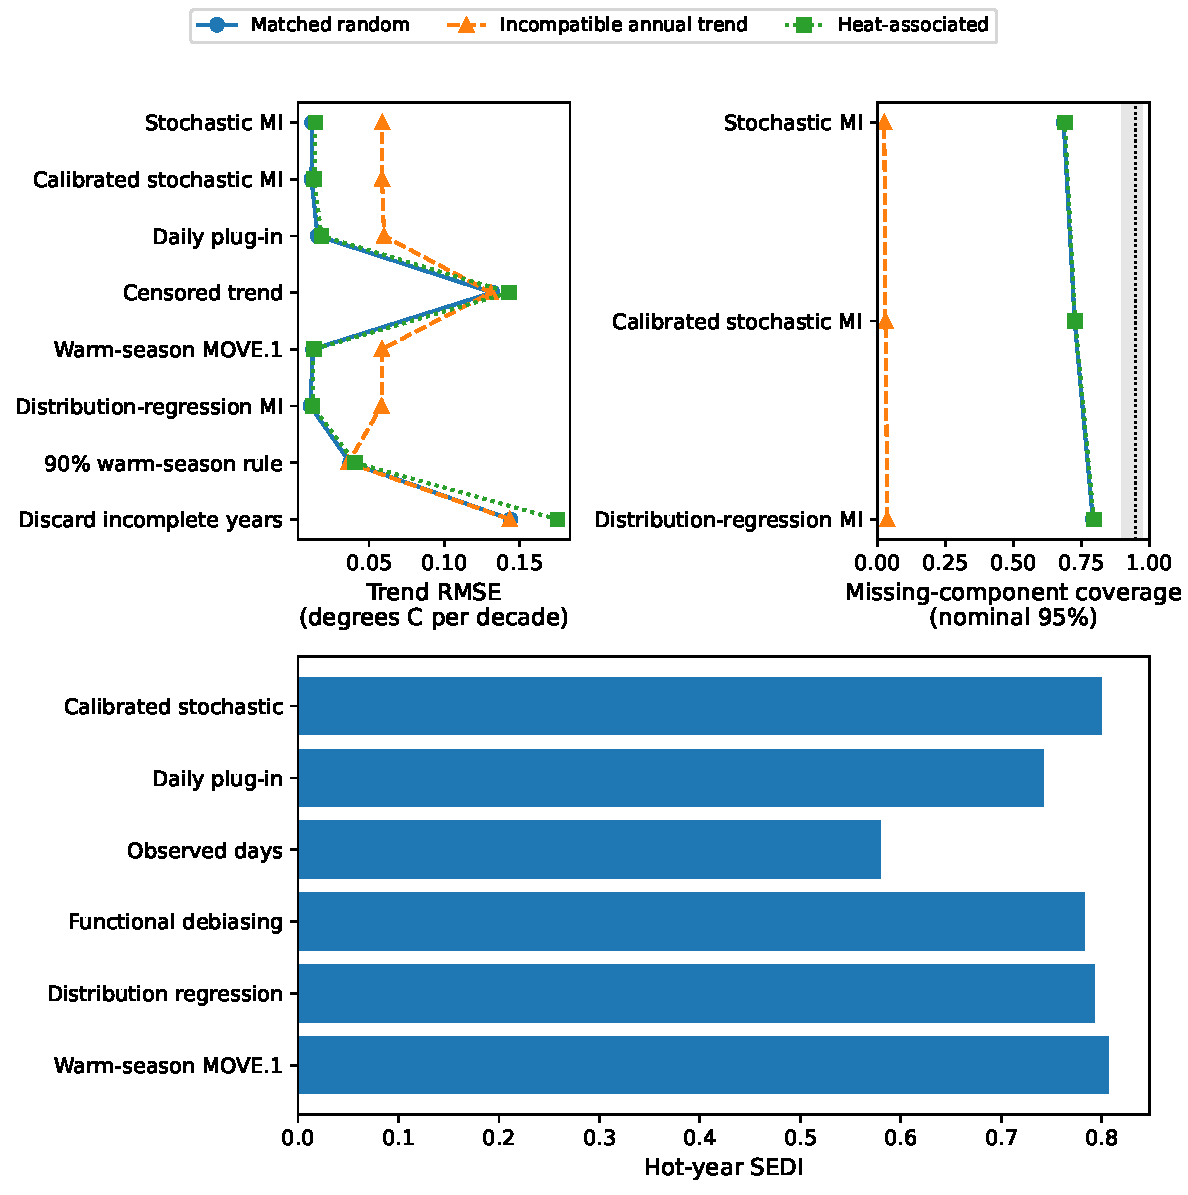
\includegraphics[width=\textwidth]{figures/review_completion/r4_6_downstream_events.pdf}\caption{Trend RMSE, missing-component interval coverage and hot-year event skill. The shaded interval is the 90--97\% coverage gate for nominal 95\% missing-component intervals. Reduced RMSE does not establish calibrated functional uncertainty. The incompatible annual diagnostic differs from the separate full daily refit.}\label{fig:downstream}\end{figure}
\bibliography{references_tr,references_review_completion}
\end{document}
